\subsubsection{Ažuriranje plana ishrane}

\begin{figure}[H]
\begin{center}
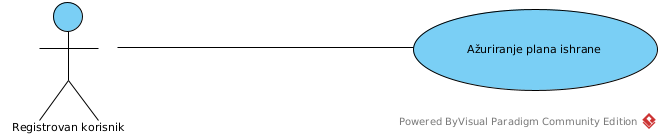
\includegraphics[width=\textwidth]{uc_update_meal_plan.png}
\end{center}
    \caption{Dijagram slučaja upotrebe ažuriranja plana ishrane}
\label{fig:UCUpdateMealPlan}
\end{figure}

\begin{itemize}
    \item Kratak opis:
        \begin{itemize}
            \item Registrovani korisnik ažurira svoj plan ishrane 
        \end{itemize}
    \item Učesnici:
        \begin{itemize}
            \item Registrovan korisnik
        \end{itemize}
    \item Preduslovi:
        \begin{itemize}
            \item Sistem je u ispravnom stanju
            \item Korisnik mora biti registrovan i ulogovan na aplikaciju
            \item Korisnik se već jednom ulogovao na aplikaciju
            \item Prva sledeća dostava narudžbine je zakazana za dalje od pet dana
        \end{itemize}
    \item Postuslovi:
        \begin{itemize}
            \item Podaci su uspešno sačuvani u bazi podataka, zakazana je dostava hrane i novac će biti skinut sa računa narednog dana
        \end{itemize}
    \item Osnovni tok:
        \begin{enumerate}
            \item Korisnik bira opciju da ažurira svoj plan ishrane
            \item Sistem prikazuje korisniku formu za izmenu plana
            \item Korisnik ažurira i potvrđuje odabir plana
            \item Sistem čuva podatke i skida novac sa korisnikovog računa narednog dana
            \item Sistem prikazuje poruku o uspešnosti 
        \end{enumerate}
    \item Alternativni tok:
        \begin{itemize}
            \item Pad sistema. Ukoliko sistem prestane sa radom u bilo kom trenutku, prelazi se na slučaj upotrebe ``Pravljenje rezervne kopije i oporavak baze podataka''.
            \item Ukoliko sistem u 4. koraku ne uspe da obavi skidanje novca sa računa, obaveštava korisnika o tome sa porukom o grešci. Proces se nastavlja u 3. koraku osnovnog toka.
        \end{itemize}
    \item Dodatne informacije:
        \begin{itemize}
            \item Moguće je ažurirati recepte koji su izabrani, ažurirati tip plana(vrsta obroka, broj ljudi i broj obroka), ažurirati adresu, datum i satnicu dostave, preskočiti dostavu za ovu nedelju i otkazati pretplatu 
        \end{itemize}
\end{itemize}

\begin{figure}[H]
\begin{center}
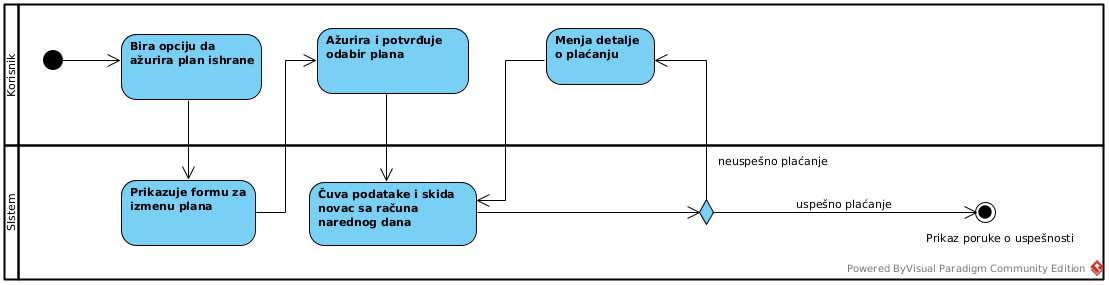
\includegraphics[width=\textwidth]{activity_update_meal_plan.png}
\end{center}
    \caption{Dijagram aktivnosti ažuriranja plana ishrane}
\label{fig:ActivityUpdateMealPlan}
\end{figure}
